\documentclass[12pt,letterpaper]{article}

% Paquetes necesarios para formato APA
\usepackage[utf8]{inputenc}
\usepackage[spanish]{babel}
\usepackage[margin=1in]{geometry}
\usepackage{setspace}
\usepackage{times}
\usepackage[style=apa,backend=biber]{biblatex}
\usepackage{csquotes}
\usepackage{fancyhdr}
\usepackage{titletoc}
\usepackage{tocloft}
\usepackage{amsmath}
\usepackage{amsfonts}
\usepackage{graphicx}
\usepackage{float}
\usepackage{caption}
\usepackage{subcaption}

% Configuración de la bibliografía
\addbibresource{MecFracII.bib}

% Configuración de página
\doublespacing
\setlength{\parindent}{0.5in}

% Configuración de encabezados
\pagestyle{fancy}
\fancyhf{}
\fancyhead[R]{\thepage}
\fancyhead[L]{MECÁNICA DE LA FRACTURA}
\renewcommand{\headrulewidth}{0pt}
\setlength{\headheight}{15.14989pt}

% Configuración del título en tabla de contenido
\renewcommand{\contentsname}{Tabla de Contenido}
\renewcommand{\refname}{Referencias}

\begin{document}

% PORTADA
\begin{titlepage}
\centering

{\Large\textbf{MECÁNICA DE LA FRACTURA II}}\\[0.5cm]
{\large Conceptos Fundamentales y Aplicaciones}\\[2cm]

{\large Presentado por:}\\[0.5cm]
{\large Gustavo Alejandro Vergara Pareja}\\%[2cm]
{\large Issa Katerine Peralta Gonzales}\\[2cm]

{\large Presentado a:}\\[0.5cm]
{\large Marco Andres Violet Lozano}\\[2cm]

{\large Universidad de Córdoba}\\
{\large Facultad de Ingeniería}\\
{\large Departamento de Ingeniería Mecánica}\\[5cm]

{\large Montería, Córdoba}\\
{\large \today}

\end{titlepage}

% TABLA DE CONTENIDO
\newpage
\tableofcontents
\newpage

% INTRODUCCIÓN
\section{Introducción}

La mecánica de la fractura es una rama fundamental de la mecánica de sólidos que estudia la propagación de grietas en materiales bajo diferentes condiciones de carga. Este documento presenta los conceptos que constituyen una extensión de los principios básicos hacia aplicaciones más complejas y especializadas.

El estudio de la mecánica de la fractura ha evolucionado significativamente desde los trabajos pioneros de Griffith (1921) y ha encontrado aplicaciones cruciales en la ingeniería estructural, aeroespacial, civil y de materiales. La comprensión de los mecanismos de fractura es esencial para el diseño seguro y eficiente de componentes estructurales, especialmente cuando estos operan bajo condiciones de carga extremas o en ambientes agresivos.

Los conceptos avanzados que se abordan en este documento incluyen la mecánica de la fractura elastoplástica, los criterios de fractura multiaxial, la fatiga y crecimiento de grietas, así como las técnicas experimentales y numéricas modernas para el análisis de la integridad estructural.

% DESARROLLO/CUERPO DEL DOCUMENTO


\section{Inestabilidad de la grieta y la curva R}

La inestabilidad de una grieta se produce cuando el avance de la fisura se vuelve incontrolable bajo una carga dada, asociado a la resistencia intrínseca del material a la propagación de la grieta. La \textit{curva R} representa la tenacidad creciente del material con el avance estable de la grieta, mostrando un equilibrio entre la energía liberada y la energía necesaria para iniciar/propagar el defecto \cite{Broek1982, Cameron2022, Jaramillo2008, AllisonBeese2022, Ponson2022}.

En otras palabras, la inestabilidad de la grieta ocurre cuando la energía elástica disponible se iguala a la energía requerida para la aparición de una grieta (Energía de superficie).
Y la curva R no es más que la representación gráfica de la resistencia del material a la propagación de una grieta en función del avance de la misma.
\vspace{1em}
\begin{figure}[H]
    \centering
    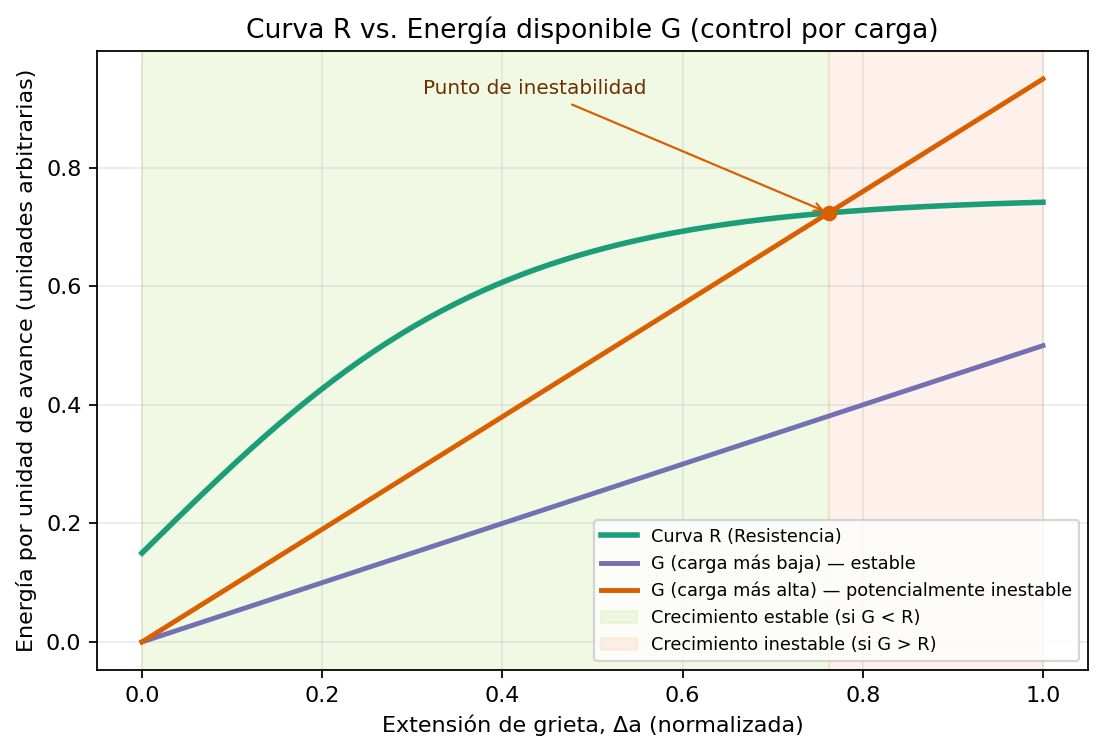
\includegraphics[width=0.8\linewidth]{aa.jpeg} % <-- sustituye por la ruta y nombre del archivo
    \caption{Esquema de elemento delgado en tensión plana.}
    \label{fig:Curva R}
\end{figure}

\section{Tensión Plana}

La condición de tensión plana se aplica a elementos delgados en los que las cargas actúan en el plano y las deformaciones fuera del plano son despreciables.
En esta condición, las tensiones fuera del plano ($\sigma_z$) son cercanas a cero, y la deformación en esa dirección ($\varepsilon_z$) puede ser significativa debido a la relación de Poisson que dice que la cara que este ortogonal a la dirección de la carga se contrae. \cite{Cameron2022, Ponson2022, Broek1982, Jaramillo2008}.
\vspace{1em}

\begin{figure}[H]   
    \centering
    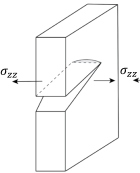
\includegraphics[width=0.3\linewidth]{BB.png} % <-- sustituye por la ruta y nombre del archivo
    \caption{Esquema de elemento delgado en tensión plana.}
    \label{fig:tension_plana}
    \caption*{Nota. Imágenes tomadas de: Coates, C., \& Sooklal, V. (2022). Modern Applied Fracture Mechanics. CRC Press.}
\end{figure}

\section{Deformación Plana}

En cuerpos con gran espesor respecto a otras dimensiones, se desarrolla una condición de deformación plana: las deformaciones fuera del plano se anulan ($\varepsilon_z \approx 0$), y el efecto triaxial en la punta de la grieta limita la plasticidad, siendo fundamental para la validez del parámetro $K_I$ \cite{Cameron2022, Ponson2022, Broek1982, Jaramillo2008}.
Los cuerpos sometidos a deformación plana serán el objeto de estudio en la MFEL principalmente.

Con la aplicación de la carga, la grieta queda restringida sin poder deformarse en una de las direcciones, dando como resultado un estado de esfuerzos triaxial en la punta de la grieta, lo que limita la plasticidad y permite el uso del factor de intensidad de esfuerzos $K_I$ para caracterizar el campo de tensiones cerca de la punta de la grieta, ya que para restringir esa deformación amerita que se induzca una tensión en la dirección z, que es la que se encuentra restringida.
\vspace{1em}
\begin{figure}[H]
    \centering
    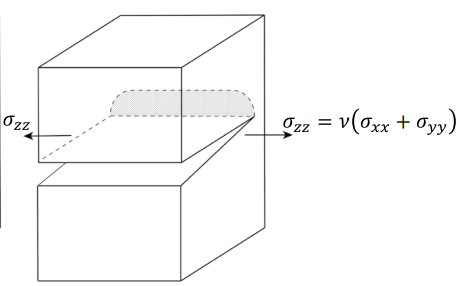
\includegraphics[width=0.4\linewidth]{ss.png} % <-- sustituye por la ruta y nombre del archivo
    \caption{Comparación de perfiles de tensiones en condiciones de deformación plana.}
    \label{fig:deformacion_plana}
    \caption*{Nota. Imágenes tomadas de: Coates, C., \& Sooklal, V. (2022). Modern Applied Fracture Mechanics. CRC Press.}
\end{figure}

\section{Factor de Intensidad en una Placa Finita}

El factor de intensidad de esfuerzos $K$ caracteriza el campo de tensiones cerca de la punta de la grieta. Es función de la geometría, tamaño de la grieta y la carga aplicada. Para una placa finita, $K = Y\sigma\sqrt{\pi a}$, donde $Y$ es el factor geométrico, $\sigma$ la tensión aplicada y $a$ la longitud de la grieta. Las tablas y gráficos de $Y$ para diversas configuraciones están recopiladas en los manuales de Tada, París y Anderson \cite{Broek1982, Cameron2022, Jaramillo2008, MechanicalBehavior2022}.
\section{Plasticidad en el Frente de Grieta}

La concentración de esfuerzos hace que la zona cercana a la punta de la grieta entre en plasticidad (zona plástica). Su tamaño se estima mediante las soluciones de Irwin y Dugdale. En deformación plana, la plasticidad es más restringida que en tensión plana. La estimación para el tamaño de zona plástica es:
\subsection*{1. Criterio de von Mises}
La tensión equivalente según von Mises está dada por:
\[
\sigma_e = \frac{1}{\sqrt{2}} \left[ (\sigma_1 - \sigma_2)^2 + (\sigma_1 - \sigma_3)^2 + (\sigma_2 - \sigma_3)^2 \right]^{1/2}
\]
La condición de fluencia ocurre cuando:
\[
\sigma_e = \sigma_{ys}
\]

\subsection*{2. Campo de tensiones cerca de la punta de la grieta (Modo I)}
El estado de tensiones en la punta de una grieta en un cuerpo elástico lineal fue formulado por George R. Irwin en 1957. La expresión analítica es:

\[
\sigma_{ij} = \left(\frac{K}{\sqrt{2\pi r}}\right) f_{ij}(\theta) + H.O.T.
\]

donde $\theta$ es el ángulo de inclinación del elemento de tensión respecto al eje de la grieta, $r$ es la distancia radial desde la punta de la grieta, $f_{ij}(\theta)$ es una función adimensional de $\theta$, y $H.O.T.$ representa términos de orden superior.

En particular:
\[
\sigma_x = \frac{K_I}{\sqrt{2\pi r}} \cos\frac{\theta}{2}\left(1-\sin\frac{\theta}{2}\sin\frac{3\theta}{2}\right)
\]
\[
\sigma_y = \frac{K_I}{\sqrt{2\pi r}} \cos\frac{\theta}{2}\left(1+\sin\frac{\theta}{2}\sin\frac{3\theta}{2}\right)
\]
\[
\tau_{xy} = \frac{K_I}{\sqrt{2\pi r}} \cos\frac{\theta}{2}\sin\frac{\theta}{2}\cos\frac{3\theta}{2}
\]

\subsection*{3. Sustitución en von Mises}
Al aplicar la ecuación de von Mises a estas tensiones, se obtiene:
\[
\sigma_e = \frac{K_I}{\sqrt{2\pi r}} \cdot g(\theta)
\]
donde $g(\theta)$ es una función que depende del ángulo $\theta$.

\subsection*{4. Igualar a $\sigma_{ys}$ y despejar $r$}
\[
\frac{K_I}{\sqrt{2\pi r}} \cdot g(\theta) = \sigma_{ys}
\]
\[
\sqrt{r} = \frac{K_I}{\sigma_{ys}\sqrt{2\pi}} \cdot g(\theta)
\]
\[
r(\theta) = \frac{1}{2\pi} \left( \frac{K_I}{\sigma_{ys}} \right)^2 [g(\theta)]^2
\]

\subsection*{5. Expresiones finales}
Para \textbf{esfuerzo plano (plane stress)}:
\begin{equation}
r_y(\theta) = \frac{1}{4\pi} \left( \frac{K_I}{\sigma_{ys}} \right)^2 \left[ 1 + \cos\theta + \frac{3}{2}\sin^2\theta \right]
\label{eq:zona_plastica_esfuerzo_plano}
\end{equation}

Para \textbf{deformación plana (plane strain)}:
\begin{equation}
r_y(\theta) = \frac{1}{4\pi} \left( \frac{K_I}{\sigma_{ys}} \right)^2 \left[ (1 - 2\nu)^2(1 + \cos\theta) + \frac{3}{2}\sin^2\theta \right]
\label{eq:zona_plastica_deformacion_plana}
\end{equation}

\subsection*{6. Aproximación clásica para $\theta = 0$}
\begin{equation}
r_p = \frac{1}{2\pi} \left( \frac{K_I}{\sigma_{ys}} \right)^2 \quad \text{(esfuerzo plano)}
\label{eq:zona_plastica_esfuerzo_plano_clasica}
\end{equation}
\begin{equation}
r_p = \frac{1}{6\pi} \left( \frac{K_I}{\sigma_{ys}} \right)^2 \quad \text{(deformación plana)}
\label{eq:zona_plastica_deformacion_plana_clasica}
\end{equation}
donde $K_I$ es el factor de intensidad y $\sigma_Y$ el límite elástico del material. \cite{Broek1982, Jaramillo2008, Cameron2022, MechanicalBehavior2022, Ponson2022}.

Así entonces, la zona plástica de la grieta actúa como un “amortiguador” que reduce la concentración extrema de esfuerzos y no la singularidad con respecto al esfuerzo que se estima, i.e.
cuanto mayor sea la zona plástica, menos dominante será el término $\left(\frac{K}{\sqrt{2\pi r}}\right)$ y la MFEL deja de ser válida.
\begin{figure}[H]
    \centering
    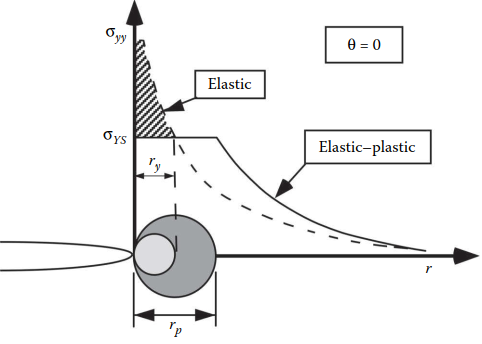
\includegraphics[width=0.7\linewidth]{ee.png} % <-- sustituye por la ruta y nombre del archivo
    \caption{Esquema de la zona plástica en la punta de la grieta.}
    \label{fig:zona_plastica}
    \caption*{Nota. Tomada de: Anderson, T. L. (2017). \textit{Fracture Mechanics - Fundamentals and Applications} (4ta ed.). CRC Press-Taylor.}
\end{figure}
\newpage
Solo serán válidas dichas soluciones cuando:

\[
a, (b-a), h \geq \frac{4}{\pi} \left( \frac{K}{\sigma_YS} \right)^2 \quad \text{(LEFM aplicable)}
\]

\begin{figure}[H]
    \centering
    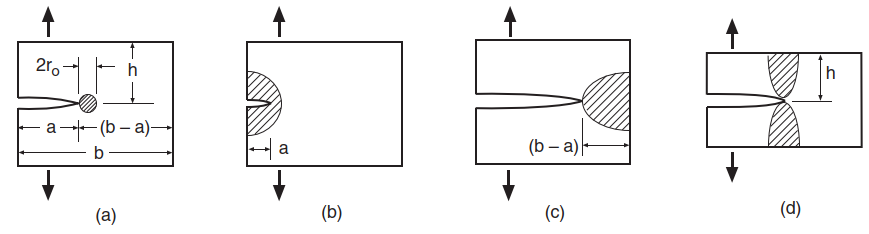
\includegraphics[width=0.9\linewidth]{ff.png} % <-- sustituye por la ruta y nombre del archivo
        \caption{Zona plástica pequeña comparada con las dimensiones planas (a), y situaciones en las que la MFEL no es válida debido a que las zonas plásticas son demasiado grandes en comparación con (b) la longitud de la grieta, (c) el ligamento sin fisurar, y (d) la altura del elemento.}
    \label{fig:zona_plastica_comparacion}
        \caption*{Nota. Tomada de: Dowling, N. E. (2022). \textit{Mechanical Behavior of Materials} (4ta ed.). Pearson.}
    \end{figure}

\section{Criterios para Determinar la Forma de la Zona Plástica}
Existen varios modelos para estimar la forma de la zona plástica en la punta de una grieta. Por criterios entendemos, las diferentes formas en las que podemos calcular y graficar la zona plástica. Por otro lado, podemos pensar en los distintos modelos y correcciones como los propuestos por Irwin, Dugdale y el enfoque basado en el J-integral. Cada uno ofrece una perspectiva diferente sobre cómo se distribuye la plasticidad alrededor de la punta de la grieta. \cite{Broek1982, Cameron2022, Jaramillo2008, MechanicalBehavior2022, Ponson2022}.
Si pensamos en los criterios para graficar la zona plástica, podemos considerar:
\begin{itemize}
    \item \textbf{Criterio de~Von Mises:} Utiliza la tensión equivalente para definir la zona plástica, considerando la combinación de tensiones principales. De este derivamos las ecuaciones~\ref{eq:zona_plastica_esfuerzo_plano} y~\ref{eq:zona_plastica_deformacion_plana}.
    \item \textbf{Criterio de Tresca:} Se basa en la diferencia máxima entre las tensiones principales para determinar la zona plástica.
    Si se utiliza el criterio de Tresca, la forma de la zona plástica resulta ligeramente diferente. A partir de los círculos de Mohr, se encuentra que la máxima tensión cortante en tensión plana es $\tau_{max} = \frac{1}{2}\sigma_1$, y en deformación plana $\tau_{max} = \frac{1}{2}(\sigma_1 - \sigma_3)$, siendo la mayor la relevante.
    
    La zona plástica según Tresca se determina como:
    
    \textbf{Tensión plana:}
    \[
    r_p = \frac{K^2}{2\pi\sigma_{ys}^2} \left[ \cos\frac{\theta}{2} \left(1 + \sin\frac{\theta}{2}\right) \right]^2
    \]
    \textbf{Deformación plana:}
    El mayor valor entre:
    \[
    r_p = \frac{K^2}{2\pi\sigma_{ys}^2} \cos^2\frac{\theta}{2} \left[ 1 - 2\nu + \sin\frac{\theta}{2} \right]^2
    \]
    y
    \[
    r_p = \frac{K^2}{2\pi\sigma_{ys}^2} \cos^2\frac{\theta}{2}
    \]
    Las zonas plásticas según Tresca suelen ser ligeramente mayores y de forma algo diferente a las obtenidas por el criterio de Von Mises.
\vspace{1em}
\begin{figure}[H]
    \centering
    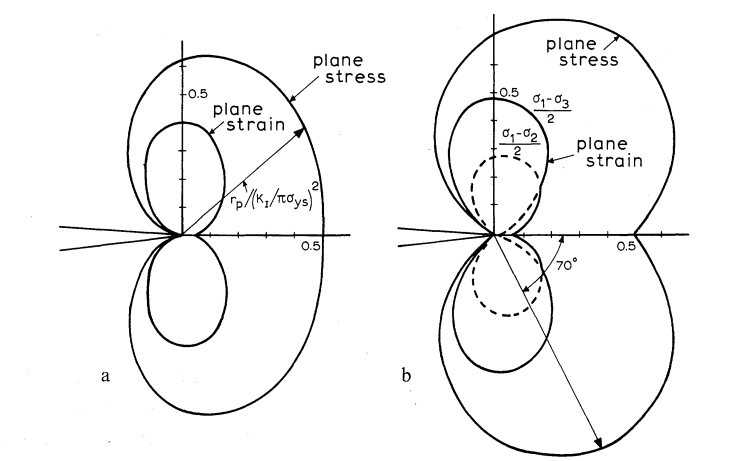
\includegraphics[width=0.8\linewidth]{gg.png} % <-- sustituye por la ruta y nombre del archivo
    \caption{Formas de la zona plástica según los criterios de Von Mises (a) y Tresca (b).}
    \label{fig:formas_zona_plastica}
\end{figure}
Ahora bien, si hablamos de los modelos para estimar la zona plástica, tenemos:
    \item \textbf{Modelo de Irwin:} Considera la zona plástica como una región semicircular delante de la punta de la grieta, con un radio proporcional a $\left(\frac{K}{\sigma_{ys}}\right)^2$.
    \item \textbf{Modelo de Dugdale:} Asume una distribución uniforme de tensión igual al límite elástico en una pequeña región delante de la punta de la grieta, formando una zona plástica rectangular.
    \item \textbf{Modelo de Dugdale:} Dugdale propone que la zona plástica delante de la grieta puede modelarse como una banda donde la tensión es constante e igual al límite elástico $\sigma_{ys}$. El tamaño de esta zona se determina igualando la apertura plástica al desplazamiento elástico en la punta de la grieta, obteniendo:

    \[
    \rho = \frac{\pi^2 \sigma^2 a}{8 \sigma_{ys}^2} = \frac{\pi}{8} \left( \frac{K_I}{\sigma_{ys}} \right)^2
    \]

    Esta ecuación es muy similar a la obtenida anteriormente Ecuación \eqref{eq:zona_plastica_esfuerzo_plano_clasica} por Irwin usando el criterio de von Mises para esfuerzo plano.

    Por ejemplo, Broek discute detalladamente los modelos de Irwin y Dugdale, mostrando cómo ambos permiten estimar el tamaño y la forma de la zona plástica en la punta de la grieta, y resalta las diferencias en los factores numéricos y supuestos físicos involucrados \cite{Broek1982}.
    \item \textbf{Enfoque del J-integral:} Utiliza el concepto de energía para definir la zona plástica, considerando la integral J alrededor de la punta de la grieta.

\end{itemize}

\section{Tablas de Factores de Intensidad}

A continuación se presentan algunas tablas y esquemas del factor geométrico $Y$ para distintas geometrías.

\begin{figure}[H]
    \centering
    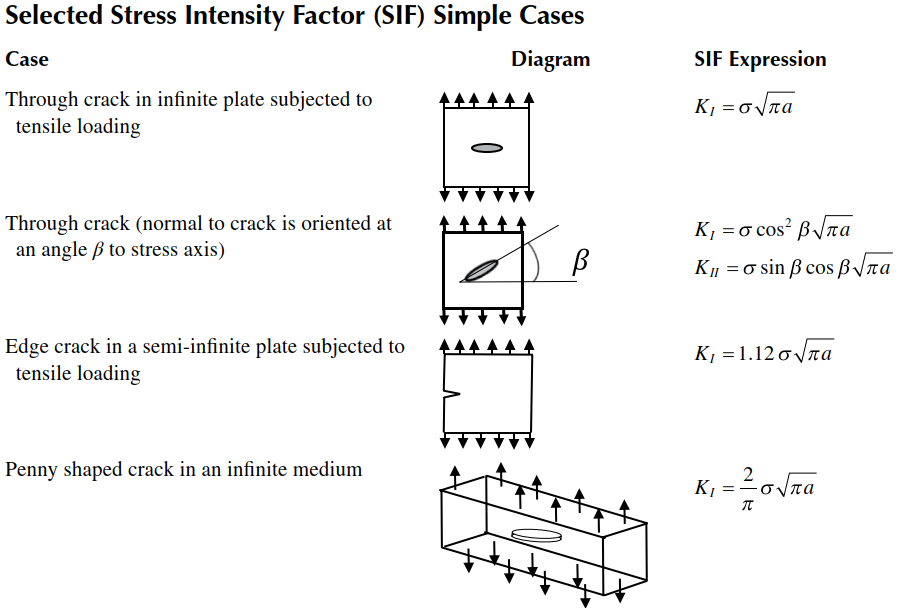
\includegraphics[width=0.65\linewidth]{cc.png} % <-- sustituye por la ruta y nombre del archivo
    \caption{Tablas y esquemas del factor geométrico $Y$ para distintas geometrías.}
    \label{fig:factor_intensidad_Y}
    \caption*{Nota. Imágenes tomadas de: Coates, C., \& Sooklal, V. (2022). Modern Applied Fracture Mechanics. CRC Press.}
    \end{figure}

\begin{figure}[H]
    \centering
    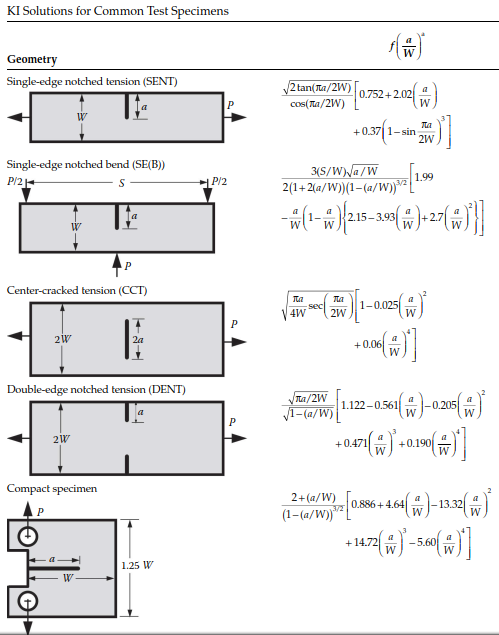
\includegraphics[width=0.85\linewidth]{d.png} % <-- sustituye por la ruta y nombre del archivo
    \caption{Tablas y esquemas del factor geométrico $Y$ para distintas geometrías (Solo modo K1).}
    \label{fig:factor_intensidad_Y2}
    \caption*{Nota. Tomada de: Anderson, T. L. (2017). \textit{Fracture Mechanics - Fundamentals and Applications} (4ta ed.). CRC Press-Taylor.}\cite{anderson2017fracture}
\end{figure}


% --------- REFERENCIAS APA 7ma ---------
\newpage
\printbibliography[title=Referencias]
\nocite{*} % Mueve este comando aquí para que todas las referencias aparezcan en la bibliografía

\end{document}